\subsection{Iterative concept}

All the approaches generally consider each frame to be independent, not related to the other ones.
This is sometimes required, since for the first processed frame no information is available.
However, since bubbles do not move much between frames, for subsequent frames an algorithm can reduce the searching window around where the bubbles could potentially be.
This knowledge can reduce the searching space for these following frames.

While the idea of searching in smaller patches may seem silly due to the results discussed in section~\ref{sec:locate:torchunfold}, here the situation is different.
Instead of searching in smaller, but meaningless and overlapping regions, this concept uses meaningful and more sparse patches.

\subsubsection{Algorithm}

The algorithm stores position, velocity and acceleration of the previously found bubbles into a list.
Velocity and acceleration are computed from the last and last two positions, respectively.
If such information is not available, the values are considered to be 0.

The different frames are processed differently, based on their index:
\begin{enumerate}
	\itemsep 0em
	\item First frame:
	      \begin{enumerate}
		      \itemsep 0em
		      \item Perform a full frame \locate*;
		      \item Add all the bubbles into the (previously empty) list.
	      \end{enumerate}
	\item All other frames:
	      \begin{enumerate}
		      \itemsep 0em
		      \item Consider the bubbles currently in the list;
		      \item Estimate their future position based on the current velocity and acceleration;
		      \item In a patch around the predicted position, perform a \locate*;
		      \item If the bubble is found, update its trajectory;
		      \item Otherwhise, if a bubble is lost for some frames, remove it from the list.
	      \end{enumerate}
	\item Every $N$ frames:
	      \begin{enumerate}
		      \itemsep 0em
		      \item Update the existing bubbles according to step 2;
		      \item Perform a full frame \locate*, to find potential bubbles that appeared in the last $N$ frames;
		      \item Add to the list the bubbles that were found by this full frame \locate*, and are not yet present in the list.
	      \end{enumerate}
\end{enumerate}

This concept is a ``meta-algorithm'', in the sense that it relies on another \locate* algorithm as a backend.
For the evaluation, multiple underying algorithm was chosen as backend.

\subsubsection{Evaluation}

Both the qualty and the speed of the meta-algorithm were worse than the original algorithm.
For example, when using the Hough algorithm (see section~\ref{sec:locate:hough}), the quality was reduced from 84\% to 43\% (figure~\ref{fig:locate:iterative}), and the speed from 55 to 15 FPS.

This meant that the divide and conquer approach was not advantageous, even if the tiles were meaningful.

\begin{figure}
	\centerline{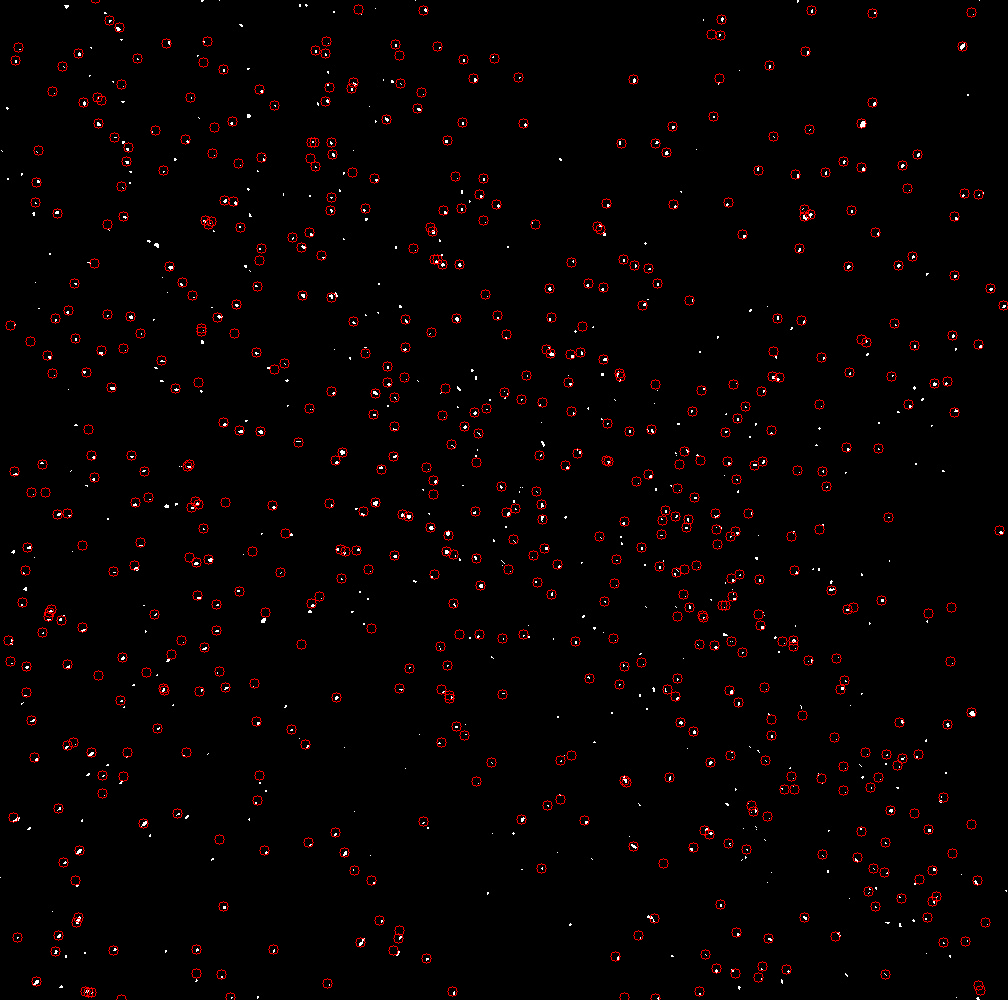
\includegraphics[width=\locateimgsize]{images/locate/iterative-Hough.png}}
	\caption{\centering Iterative concept with Hough backend's result}
	\label{fig:locate:iterative}
\end{figure}
